In the following, the necessary settings and how they were determined are described. Important parameters are discussed and the used values are explained. The directory structure of the simulations, primarily dictated by \texttt{OpenFOAM}, is depicted below. The folder \texttt{0.orig} contains the files required for initializing the simulation. At the start of the simulation initialization, a folder \texttt{0} is automatically created based on the files in this directory, containing the initialized fields necessary for the simulation. The \texttt{constant} directory contains files defining physical properties and how they should be handled during the simulation. The \texttt{system} folder has files that define the simulation itself, including the geometry and meshing, the duration of the simulation, and, in the case of the diffuse interface, its initialization.

In the following, all important settings are presented and explained briefly. However, it is assumed that the reader is familiar with the basic settings of \texttt{OpenFOAM}.

\section{Geometry and Discretization}

The geometry of the capillary is assumed to have a reservoir of water, as seen in Figure \ref{fig: Capillary Geometry}, which flows into the capillary due to surface effects. By assuming that some of the water is already in the capillary, the simulated geometry only sets the boundary condition so that the water can flow in from this reservoir. This way, the reservoir does not have to be modeled and discretized. The dimensions of the capillary result from the perspective that the simulation of the capillary should also be compared with experiments in the future. Therefore, more complex geometries were also simulated but are not part of this work. As can be seen, it is a capillary with only a $6nm$ diameter. To the best of our knowledge, a simulation of such a small capillary has not been done using the phase-field method.

\begin{figure}[h]
\centering
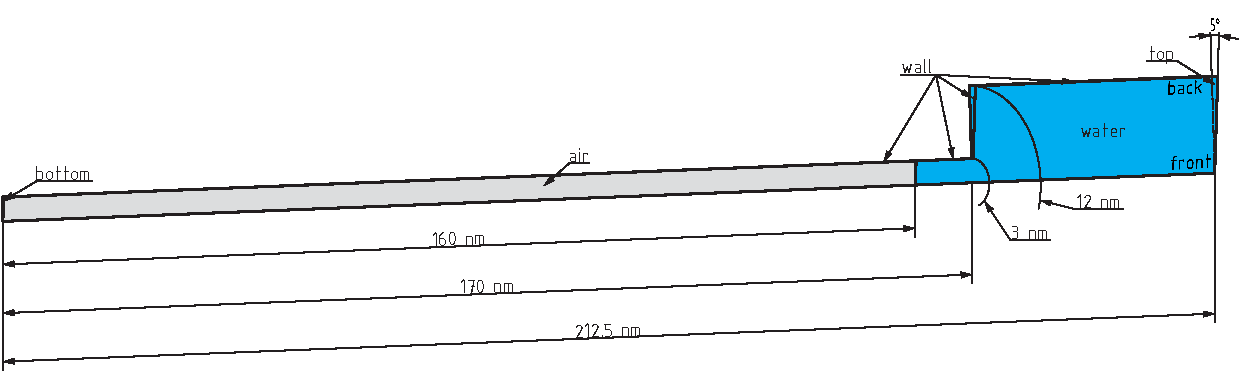
\includegraphics[width=.95\textwidth]{Pictures/Cap_5DEG.pdf}
\caption{Schematic of used Capillary}
\label{fig: Capillary Geometry}
\end{figure}

As indicated in the image, not the entire capillary is simulated, but only a segment of the capillary, called a \textit{wedge}. It is assumed that the flow in the capillary is axisymmetric, which significantly simplifies the simulation since fewer elements are required for discretization, as only a $5^{\circ}$ segment of the capillary is being simulated. A necessary condition for simulating the wedge is that it can only have one element in the radial direction.

The discretization of the geometry was chosen so that the elements have an edge length of $0.3nm$ to $0.4nm$. Due to the assumptions, the simple geometry can easily be directly defined in a \texttt{blockMeshDict} file. The geometry is described in terms of vertices and reduced to blocks. To define the boundary conditions on the surfaces, they also need to be defined and named therein. Figure \ref{fig: Capillary Geometry} shows the named surfaces besides the geometry. The \texttt{front} and \texttt{back} surfaces are opposing surfaces of the wedge and must receive corresponding boundary conditions. The \texttt{wall} surfaces are impermeable, and \texttt{top} or \texttt{bottom} are surfaces that allow flow. To create the \texttt{blockMeshDict} file, a Python script was developed, which, based on the capillary diameter and length, creates a file with the surface names depicted in Figure \ref{fig: Capillary Geometry}. Boundary conditions must be defined for these, listed in the following Table \ref{tab: BoundaryConditions}.

\begin{table}[h]
    \centering
        \caption{Relevant boundary conditions for the wall}
        \label{tab: BoundaryConditions_wall}
        \begin{tabular}{lll}
            Parameter & Value \\ \hline
            Order parameter $C$ & \texttt{equilibriumPhaseContactAngle}     \\
            Equilibrium contact angle $\theta_{\mathrm{e}}$ & $15^{\circ}$, $45^{\circ}$, $75^{\circ}$\\
            Chemical potential $\phi$   & \texttt{zeroGradient}        \\ 
            Velocity $\mathbf{u}$ &   $\mathbf{u_{\mathrm{w}}} = 0$\\
            Pressure $p$&  \texttt{fixedFluxPressure} \\
        \end{tabular}
\end{table}

For the order parameter $C$, the equilibrium boundary condition is assumed, and the equilibrium contact angle is specified as $15^{\circ}$, $45^{\circ}$, or $75^{\circ}$ for each of the three simulations with this geometry. For additional simulations, apart from the mentioned equilibrium condition \texttt{equilibriumPhaseContactAngle}, an imbalance according to \ref{sec: nonEquiBC} is assumed. For this, the boundary condition should be changed to \texttt{outOfEquilibriumPhaseContactAngle} and a value for $\Gamma_{\mathrm{w}}$ should be specified. The gradient of the chemical potential on the wall is set to zero, as is the wall's velocity. The pressure boundary condition is chosen as \texttt{fixedFluxPressure} to adjust the pressure gradient so that the mass flow at the boundary matches the specified velocity at the wall. A \texttt{zeroGradient} boundary condition and a pressure of $0$ Pa are also applied at the inlet and outlet of the capillary.

Furthermore, water and air at $25^{\circ}$ Celsius are assumed as the media for the simulation. This results in the material properties shown in Table \ref{tab:physicalProperties_CaseSetup}.

\begin{table}[h]
    \centering
    \caption{Physical properties}
    \label{tab:physicalProperties_CaseSetup}
    \begin{tabular}{lll}
    Fluid & Density $\frac{kg}{m^3}$ & Kinematic viscosity $\frac{m^2}{s}$ \\ \hline
    Water & $1000$                     & $1.00E-06$                          \\
    Air   & $1$                        & $1.00E-05$                          \\ 
    \end{tabular}
    \end{table}

The surface tension for a water-air interface at $25^{\circ}$ Celsius is given as \(0.072 N/m\). The interface thickness \( \epsilon \) was chosen to be approximately \(1.7 nm\) \cite{bagheriInterfacialRelaxationCrucial2022}, corresponding to the physical interface thickness. Thus, all settings directly derived from the geometry or the materials have been determined, and further parameters necessary for the simulation will follow.

\section{Simulation Parameters}
The mobility ($\kappa$) is a challenging factor to determine in the phase-field simulation. Jacqmin \cite{jacqmin1999CalculationTwoPhaseNavier} suggested an asymptotic behavior for \( \kappa \) of 
\begin{equation}
    \kappa = \mathcal{O}(\epsilon^{\delta})
\end{equation}
and showed that \( 1 \leq \delta < 2 \). Unfortunately, there is no concrete calculation method for the mobility $\kappa$ and the wall relaxation factor $\Gamma_{\mathrm{w}}$ so far.

For the assumption of two immiscible fluids ($mu_{\mathrm{A}}, mu_{\mathrm{B}}$) with different viscosities, the surface-interpolated dynamic laminar viscosity $mu_{\mathrm{f}}$ in \texttt{phaseFieldFoam} is calculated using three viscosity models. The choice of the viscosity model can significantly influence the results \todo{ref to image or chapter}. The three methods are $\mu_{\mathrm{f}}^{(S)}$ (serial/arithmetic), $\mu_{\mathrm{f}}^{(\mathrm{P})}$ (parallel/harmonic), and $\mu_{\mathrm{f}}^{(\mathrm{B})}$ (blended) and are defined as

$$
\begin{aligned}
&\mu_{\mathrm{f}}^{(S)} =\frac{\hat{\overline{c}}_{\mathrm{f}}+1}{2}\:\mu_{\mathrm{B}}-\frac{\hat{\overline{c}}_{\mathrm{f}}-1}{2}\:\mu_{\mathrm{A}},  \\
&\mu_{\mathrm{f}}^{(\mathrm{P})} =\frac{\mu_{\mathrm{A}}\mu_{\mathrm{B}}}{\mu_{\mathrm{f}}^{(\mathrm{S})}},  \\
&\mu_{\mathrm{f}}^{(\mathrm{B})} =\eta_{\mathrm{f}}\:\mu_{\mathrm{f}}^{\mathrm{(P)}}+(1-\eta_{\mathrm{f}})\:\mu_{\mathrm{f}}^{\mathrm{(S)}}.
\end{aligned}
$$
With $\eta_{\mathrm{f}}$ as a blending factor \cite{holzinger2021DirectNumericalSimulation}. The method to use is set in the \texttt{constant/transportProperties} file based on the chosen method.

For initializing the diffusive interface, the \texttt{funkySetFields} or \texttt{funkySetBoundaryField} methods are used. Here, the position and shape of the interface must be specified via a defining function. The variation of the order parameter normal to the interface is defined by the equation \ref{eq: InterfactialNormalDirProfile} introduced in Section \ref{sec: DiffusiveInterface}. As the interface is assumed to be planar at the start of these simulations, it is sufficient to only specify the position of the interface.

\section{Evaluation Methods}
For the evaluation of the simulation, the application \texttt{paraview} was used, among other tools. All images of the simulation were generated using it. However, the evaluation and representation of derived or calculated quantities in diagrams were produced using the Python library \texttt{Matplotlib}. A script was written for this purpose that gathers the results from the function objects and, if necessary, performs calculations with them.

With the help of \textit{function objects}, data can be captured during the running simulation. \texttt{phaseFieldFoam} already provides several functions for reading the simulation, which are also used here. These have to be integrated and configured in the \texttt{controlDict} file. \todo{maybe name some?}

For instance, to analyze the viscous forces acting within the water column, we need the total viscous dissipation force in that water column exported via such function objects. We obtain this when integrating the divergence of the viscous stress tensor $\tau$ from Equation \ref{eq: NSEChanged} over the domain.

\begin{equation}
    \label{eq: totalViscForce}
    \mathrm{F}_{\mathrm{visc}}^{\mathrm{total}} = \int_{\Omega} \mathrm{f}_{\mathrm{visc}}^{\mathrm{total}} dV = \int_{\Omega} \nabla \cdot \tau dV.
\end{equation}


\subsection{Contact Angle measurement}
\label{sec: CA_Measurement}

The actual contact angle during the simulation is of interest for several reasons. Firstly, to determine to what extent the simulation evolves over time and approaches equilibrium, and secondly, to determine the forces at play. However, measuring the contact angle is not trivial \cite{carlson2011DissipationRapidDynamic}. Several approaches can be pursued. In this work, three different approaches were chosen for evaluation. It is assumed that the meniscus in the capillary forms a circular segment. Then, with knowledge of the position of the interface at the wall and axis of the capillary, the contact angle can be calculated.
\begin{figure}[h]
    \centering
    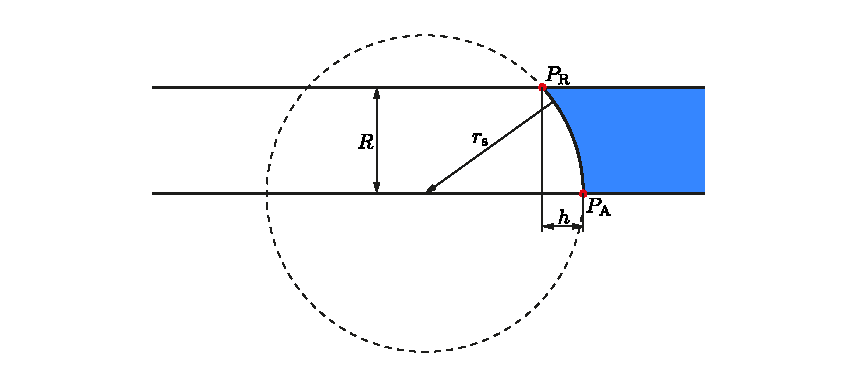
\includegraphics[width=.95\textwidth]{Pictures/RadiusCalc.pdf}
    \caption{Schematic of capillary with relevant dimensions for the calculation of radius and first method of contact angle computation}
    \label{fig: RadiusCalc}
\end{figure}
Figure \ref*{fig: RadiusCalc} illustrates the geometry of the capillary with the relevant dimensions. The points \(P_{\mathrm{R}}\) and \(P_{\mathrm{A}}\) are the intersections of the interface with the capillary wall and the axis of rotation, respectively. If these points are known, the height \(h\) of the spherical segment can be calculated, and subsequently, the radius of the sphere \(r_{\mathrm{S}}\), using the already known capillary radius \(R\). The dashed line indicates that the radius of the sphere may not necessarily match that of the capillary. The contact angle can be calculated without knowledge of the radius, but it was introduced early for later calculations. To calculate the contact angle, knowing the height \(h\) and the capillary radius is sufficient. The contact angle is then given by:
\begin{equation}
    \theta = 90^{\circ}- 2\tan^{-1}\left(\frac{h}{R}\right) 
\end{equation}
The radius is derived from:
\begin{equation}
    r_{\mathrm{S}} = \frac{R^2}{2h}+\frac{h}{2}.
\end{equation}

The other two methods used are essentially the same, only different positions are used to calculate the angle. As shown in Figure \ref{fig: CA_Method2}, a cut is simply made along the dashed line, and then a triangle is formed, resulting in the contact angle given by:
\begin{equation}
    \theta = \tan^{-1}\left(\frac{h_{\mathrm{cut}}}{h}\right)
\end{equation}

\begin{figure}[h]
    \centering
    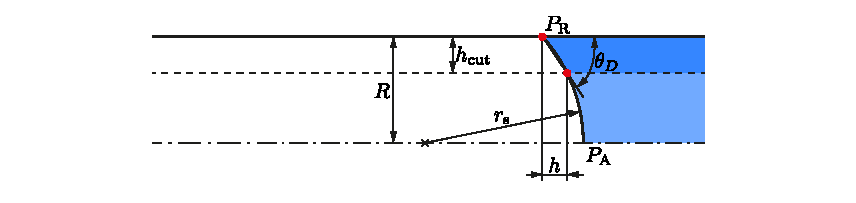
\includegraphics[width=.95\textwidth]{Pictures/CA_CALCMEthod2.pdf}
    \caption{Schematic of capillary with relevant dimensions for the calculation using the second method of contact angle computation}
    \label{fig: CA_Method2}
\end{figure}



\section{Model Calibration}
Many of the mentioned parameters, as already mentioned, are difficult to define. Therefore, to determine them, simulations were conducted in which individual parameters were varied. To determine the necessary discretization, a mesh study was conducted. The results for the used mesh and for a more refined mesh with double resolution are presented in Figure \ref*{fig: Mesh_Study}. It is evident that the results differ only slightly from each other. The computational grid used consists of \texttt{4250} cells. \todo{image MeshStudy}

\begin{figure}[h]
    \centering
    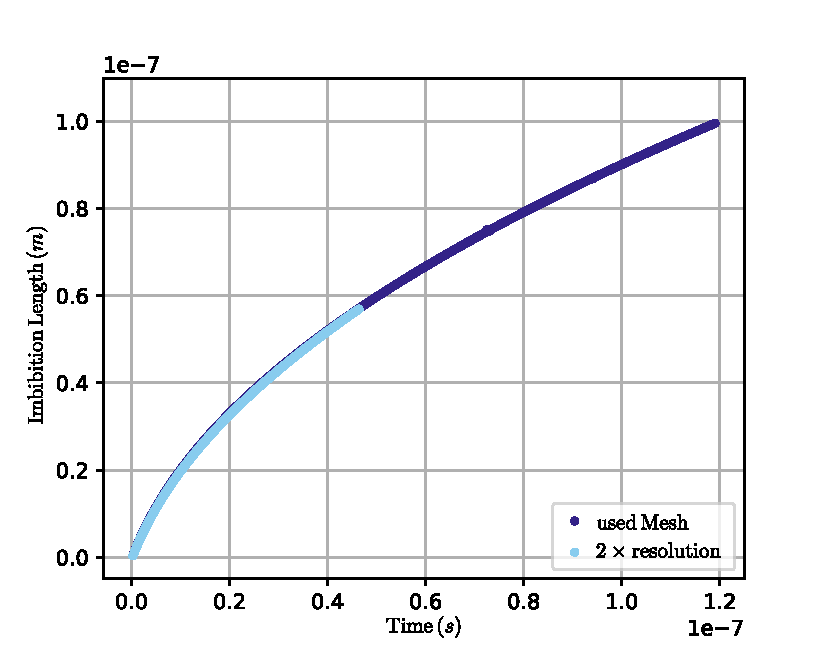
\includegraphics[width=.95\textwidth]{Pictures/Mesh_Study.pdf}
    \caption{Results of the mesh study for the used and a more refined mesh. Here the imbibition height is plotted over time.}
    \label{fig: Mesh_Study}
\end{figure}

Due to the small computational mesh, adaptive mesh refinement was not utilized. 
Since mobility is a phenomenological parameter, it's difficult to predict, and there are only recommendations. Therefore, several simulations were conducted in this area as well, and a value was agreed upon that delivers physical results while simultaneously reducing interfacial diffusion. For the subsequent simulations, a value of \(\kappa = 1.6 \times 10^{-18}\) was used.
The \texttt{blended} model was employed as the viscosity model. One advantage of this method is that the blending occurs based on the direction of velocity flows. Nonetheless, simulations were also performed to evaluate the different models.
To assess the effects of various viscosity models, simulations were also conducted here. \todo{visc Study and why we used harmonic}
Considering the dimensions of the capillary and the fluids, it's expected that the influence of gravity is negligible. This was confirmed by separate simulations, although due to the limited significance of a presentation, it's not further elaborated on here.

Throughout this work, several simulations and studies were conducted, which were ultimately not pursued further. However, some of these efforts were essential to determine the simulation parameters. This includes simulations such as the investigation of \textit{mobility} or \textit{courant number} and the various \textit{viscosity schemes}. Simulations with different discretizations of the computational domain, as well as the use of adaptive mesh refinement (AMR), were carried out. Yet, there were also simulations that did not directly contribute to determining the parameters of the simulation. This includes, for instance, simulations that took into account the \textit{pinning} effect, which is not mentioned in this work, or geometries that, despite simplifications, are closer to reality. However, these simulations will not be further considered in this work.

